\section{TTS}
\label{sec:tts}
Compared with our ASR and Realtime speech models, the distinctive aspect of StepAudio 2.5 TTS is that it completely eliminates the encoder-adapter module and relies solely on the LLM backbone for modeling. Audio tokens are treated as a new “language” within the language modeling framework, allowing speech synthesis to be reformulated as a pure next-token prediction (NTP) task. Under this paradigm, the key challenge becomes to learn effective alignment between text and audio representation spaces.
\subsection{Training Pipeline}
\label{sec:pipeline}


After pre-training, the model establishes a shared representation space between text and audio, enabling unified cross-modal modeling. Building upon this foundation, SFT further aligns text descriptions with their corresponding audio token sequences, allowing the model to generate speech conditioned on natural language instructions. Reinforcement learning is then introduced to improve alignment in scenarios where instructions become more complex, abstract, or highly context-dependent, thus improving the model’s ability to faithfully capture nuanced semantic intent in generated speech.


\textbf{SFT}
To enable the model to support both global- and inline-level controllability over arbitrary speakers, we adopt zero-shot voice cloning TTS as the primary objective during supervised fine-tuning. In the first stage, we conduct large-scale zero-shot TTS training with global instruction supervision, enabling the model to learn coarse-grained control over speaker characteristics, speaking style, and overall prosodic attributes. Building upon this capability, we further train the model using high-quality in-house speech data annotated with both global and inline instructions, thereby enabling fine-grained control at both the utterance and segment levels. Through this two-stage SFT pipeline, the model achieves an initial alignment between textual control instructions and their corresponding audio realizations, supporting both global instruction following and inline expressive control in TTS generation.

\textbf{Reinforcement Learning}
During the RL stage, we apply human feedback reinforcement learning (RLHF) to further align the generated audio tokens with textual descriptions based on human preferences. This process improves the model’s ability to interpret complex and expressive instructions, while simultaneously improving the naturalness, expressiveness, and overall perceptual quality of the synthesized speech. 

We first train a Generative Reward Model (GRM), denoted as $r_\phi$. For each prompt $x$, the training data provides a high-quality reference response $y^*$. During training, the policy model $\pi_\theta$ generates a candidate response $y$, and the GRM evaluates the relative quality of $y$ against the reference response $y^*$ under the same prompt $x$, producing a pairwise scalar preference score. The final reward used for policy optimization is obtained by applying a reward-shaping transformation to this score:

\begin{equation}
r_{hf}(x, y, y^*) = s\!\left(r_\phi(x, y, y^*)\right),
\end{equation}

where $r_\phi(x, y, y^*)$ denotes the GRM score relative to the reference response and $s(\cdot)$ denotes the transformation of the reward.


\subsection{SFT Data}
\label{sec:SFT-data}
Our SFT data consist of two categories: model-synthesized data and recorded speech data. All data used for global instruction control is synthesized using the Step-Audio-EditX~\citep{yan2025stepaudioeditxtechnicalreport} model. Owing to the strong compositional editing capabilities of Step-Audio-EditX across diverse speaking styles and emotional attributes, we are able to generate large-scale speech data with rich and highly diverse stylistic and emotional variations for global instruction supervision.

In contrast, the recorded speech data is primarily used for joint global and inline control, enabling fine-grained hierarchical expressive modeling. The detailed data construction pipeline is described below.

For internal recordings with clear dialogue context, speaker information, or available scripts, we adopt the annotation pipeline of Emotional-Context-Speech \footnote{https://huggingface.co/Insects/Emotional-Context-Speech}. The main change is the annotation target. Instead of producing structured context-aware labels, we generate two forms of natural-language supervision for zero-shot TTS: (1) a global control description for the whole utterance, and (2) inline expression descriptions for local text spans.

Following the source pipeline, we first transcribe the recordings with Whisper-Large-v3. We then use the Montreal Forced Aligner to obtain word-level timestamps and segment the recordings into utterance-level samples. We remove samples with severe alignment errors, incomplete transcripts, or very short duration. For each retained utterance, we collect contextual metadata, including dialogue history or script context. This contextual information is used during annotation.

Following Emotional-Context-Speech, we extract and discretize prosodic features, including F0, speech rate, pause statistics, spectral centroid, root mean square (RMS) energy, MFCC variance, and harmonic-to-noise ratio (HNR). We concatenate these tokenized acoustic features with the transcript and contextual metadata, and feed them to the annotating LLM.

Given the transcript, contextual metadata, and quantized acoustic features, the LLM produces two annotation outputs. The first is a global control description, which summarizes the overall speaking style, prosodic pattern, and affective state of the whole utterance. The second is an inline expression description, which inserts local directives into the text to mark span-level expressive behavior. These two outputs provide supervision for utterance-level control and mixed expression control in zero-shot TTS.

Before model training, we further verify the transcription accuracy of the segmented utterances by cross-checking their transcripts with the outputs of our ASR models. Segments with substantial transcription mismatch are discarded.


\subsection{Evaluation}
Effectively evaluating the diverse capabilities of modern TTS systems remains a challenging problem. Traditional objective metrics, such as character error rate (CER) and speaker similarity, often exhibit inherent bias when applied to LLM-based speech generation models. For instance, ASR-based metrics tend to become unreliable in the presence of rich paralinguistic phenomena, while embedding-based speaker verification models typically discard high-frequency acoustic details and fail to accurately capture similarities in prosody, speaking style, and expressive characteristics.

Similarly, LLM-as-a-judge approaches still struggle to reliably assess prosodic quality and complex emotional expression. Subjective MOS evaluation also presents significant limitations, as it requires highly trained annotators and often suffers from inconsistencies in scoring criteria across evaluators.

Considering these limitations, we adopt an arena-style pairwise evaluation framework, in which models are compared via pairwise preference judgments, and their overall performance is measured by aggregated win rates. To ensure evaluation reliability, we invest substantial effort in standardizing the evaluation protocol and improving inter-rater consistency among human evaluators.

Specifically, we proceed as follows: (1) We first conduct a listening sensitivity screening using a small set of audio samples to select qualified evaluators. Once the evaluation task begins, the set of evaluators remains fixed, and all evaluations must be completed continuously within the same evaluation period. (2) During the evaluation process, we ensure randomness in both the selection of model audio pairs and the ordering of evaluation positions, and we additionally require evaluators to provide reasons for their preference judgments. (3) We perform periodic spot checks during the evaluation process and intervene promptly when significant deviations are observed to maintain inter-rater consistency. After the full evaluation is completed, we further review cases with large discrepancies across evaluators and conduct additional verification to ensure the reliability of the final results.


\begin{figure}[h]                                    
\centering                               
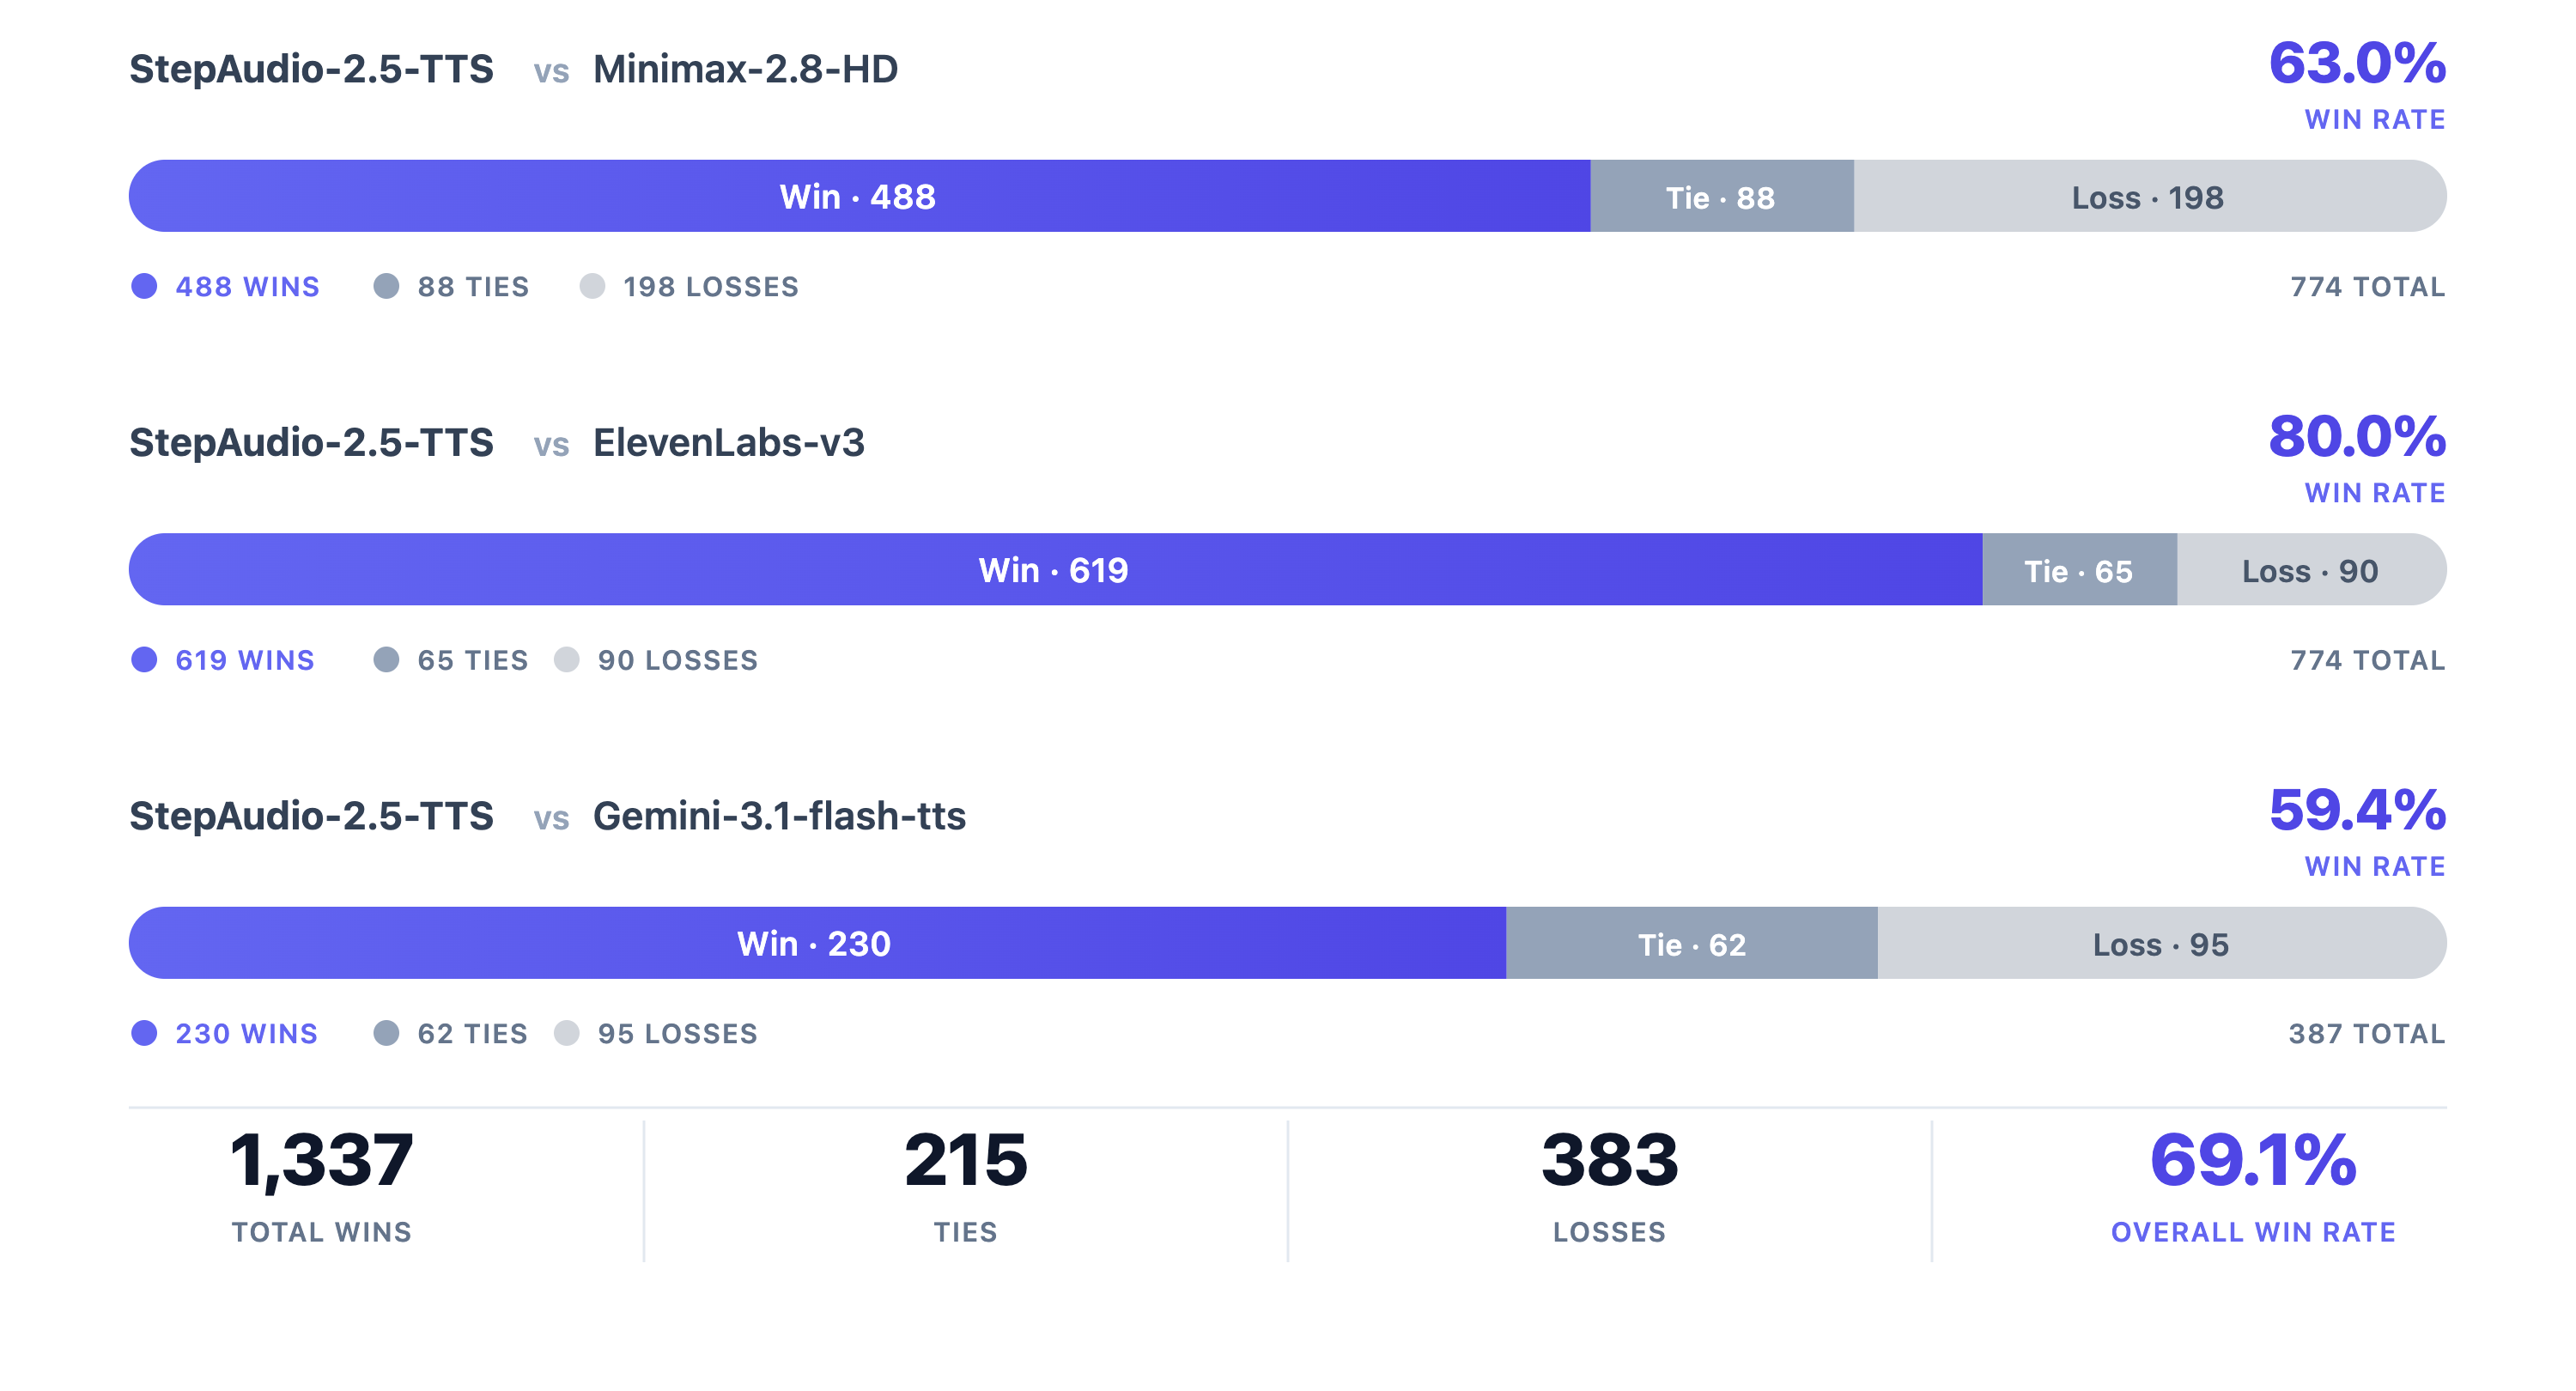
\includegraphics[width=1.0\linewidth]{figures/stepaudio25-tts-arena.png}   
\caption{Arena Win Rates of \textit{StepAudio-2.5-TTS}.} 
\label{fig:tts_arena}                                
\end{figure}  

Finally, we select three leading models with controllable generation capabilities—\textit{MiniMax-2.8-HD}, \textit{Elevenlabs-v3}, and \textit{Gemini-3.1-Flash-TTS}. For each model, we adopt its officially recommended optimal voice preset and conduct arena-based evaluation using 774 prompts.

The results in Fig.~\ref{fig:tts_arena} show that \textit{StepAudio-2.5-TTS} achieves 67.6\% overall win rate in pairwise evaluations against three strong TTS baselines, with consistent gains across all comparisons.
